\documentclass[11pt]{article}
\usepackage[utf8]{inputenc}
\usepackage[T1]{fontenc}
\usepackage{geometry}
\usepackage{amsmath}
\usepackage{amssymb}
\usepackage{booktabs}
\usepackage{hyperref}
\usepackage{enumitem}
\usepackage{tikz}
\usetikzlibrary{arrows.meta,positioning,shapes.geometric,fit}
\geometry{margin=1in}

\title{Methodology: CINeMA-Bone Fracture Atlas Project}
\author{Project Documentation}
\date{\today}

\begin{document}
\maketitle
\tableofcontents

\section{Goal and High-Level Idea}
The goal is to learn a \textbf{continuous 3D population atlas} of proximal humerus shape from fragmented fracture data, and then use that atlas to estimate where fractures most frequently occur.

The model learns a function that answers this question:
\begin{quote}
``Given a 3D coordinate and a subject identity representation, what is the SDF value at that coordinate?''
\end{quote}

This is done with an \textbf{auto-decoder} setup:
\begin{itemize}[leftmargin=*]
    \item one shared neural decoder for all subjects,
    \item one learnable latent code per subject,
    \item one learnable rigid transform per subject.
\end{itemize}

\section{End-to-End Pipeline}
The implemented pipeline has four stages:
\begin{enumerate}[leftmargin=*]
    \item \textbf{Preprocessing}: STL fragments $\rightarrow$ normalized SDF volumes.
    \item \textbf{Atlas Training}: jointly optimize decoder weights, subject latent codes, and subject rigid transforms.
    \item \textbf{Atlas Inference}: decode the population mean latent into a canonical atlas SDF and mesh.
    \item \textbf{Fracture Mapping}: compare each subject to atlas in atlas space and accumulate fracture-density statistics.
\end{enumerate}

\section{Data Representation and Preprocessing}
\subsection{Input Data}
Raw input is a directory of STL files grouped by subject folders:
\begin{itemize}[leftmargin=*]
    \item \texttt{patient\_XX}: clinical fractured subjects,
    \item \texttt{GT XX}: reconstructed/ground-truth subjects,
    \item \texttt{template\_control}: template reference.
\end{itemize}

Implementation: \texttt{data\_loading/prepare\_data.py}.

\subsection{Fragment Fusion and Normalization}
For each subject:
\begin{enumerate}[leftmargin=*]
    \item Load all STL fragments with \texttt{trimesh}.
    \item Concatenate fragments into one mesh.
    \item Center mesh around its vertex mean.
    \item Scale mesh to fit approximately into normalized coordinate cube $[-1,1]^3$.
\end{enumerate}

Implementation: \texttt{data\_loading/mesh\_to\_volume.py}.

\subsection{Voxelization and Signed Distance Field}
Each normalized mesh is converted to occupancy and then to SDF using distance transforms:
\begin{equation}
\mathrm{SDF}(x)=d_{\text{outside}}(x)-d_{\text{inside}}(x).
\end{equation}
Sign convention:
\begin{itemize}[leftmargin=*]
    \item $\mathrm{SDF}<0$: inside bone,
    \item $\mathrm{SDF}=0$: surface,
    \item $\mathrm{SDF}>0$: outside bone.
\end{itemize}
Each subject is saved as \texttt{subject\_id\_sdf.npy}. Metadata and train/validation split files are also created.

\section{Training Dataset and Sampling Strategy}
Implementation: \texttt{data\_loading/dataset.py}.

The network is not trained on full dense volumes directly. Instead, per subject, it samples coordinate-value pairs:
\begin{equation}
\{(x_n, s_n)\}_{n=1}^{N}, \quad x_n\in[-1,1]^3,
\end{equation}
where $s_n$ is the ground-truth SDF at that coordinate.

\subsection{Why Sampling?}
Sampling is memory-efficient and focuses training on geometrically important regions.

\subsection{Hybrid Sampling}
For each subject and epoch:
\begin{itemize}[leftmargin=*]
    \item A fraction is sampled near the surface ($|\mathrm{SDF}|<\tau$).
    \item The rest is sampled uniformly in the cube.
\end{itemize}
This balances boundary accuracy and global shape consistency.

\section{Model Components (Detailed)}
\subsection{Auto-Decoder: What It Means Here}
Unlike an encoder-decoder model, there is \textbf{no encoder network} that reads a subject image. Subject identity is represented by optimized latent variables directly.

Learned variables are:
\begin{itemize}[leftmargin=*]
    \item global decoder parameters $\theta$,
    \item subject latent code $z_i$ for each subject $i$,
    \item subject rigid transform parameters $p_i$ for each subject $i$.
\end{itemize}

For a coordinate $x$ belonging to subject $i$:
\begin{equation}
\hat{s}=f_\theta\big(\mathcal{T}(x; p_i),\ z_i,\ c_i\big),
\end{equation}
where $c_i$ is optional condition vector (disabled by default in current config).

\subsection{Latent Codes: Intuition and Mechanics}
\textbf{What is a latent code?}
A latent code is a compact subject-specific parameter tensor that stores how subject $i$ deviates from the average shape.

\textbf{In this project:}
\begin{itemize}[leftmargin=*]
    \item latent shape is \texttt{[128, 3, 3, 3]} per subject,
    \item this is a low-resolution 3D feature grid, not a single vector,
    \item it is learnable and updated by backpropagation during training.
\end{itemize}

\textbf{How it affects prediction:}
\begin{enumerate}[leftmargin=*]
    \item The latent grid is optionally passed through a 3D conv modulator.
    \item At each query coordinate, trilinear interpolation extracts a local feature vector from that latent grid.
    \item That feature vector modulates SIREN layers (FiLM-style) and changes output shape locally.
\end{enumerate}

Interpretation:
\begin{itemize}[leftmargin=*]
    \item decoder $f_\theta$ learns shared anatomy rules,
    \item $z_i$ captures subject-specific morphology.
\end{itemize}

\subsection{Rigid Transform Parameters}
Each subject has a learnable transformation embedding (6-DoF):
\begin{itemize}[leftmargin=*]
    \item first 3 values: rotation (axis-angle),
    \item next 3 values: translation.
\end{itemize}

The function \texttt{embed2affine()} converts this into $(R_i, t_i)$, then coordinates are transformed as:
\begin{equation}
x' = R_i x + t_i.
\end{equation}
This lets the network align each subject into a common atlas coordinate system while learning shape.

\subsection{Decoder Network: SIREN with Modulation}
Implementation: \texttt{models/siren.py}, \texttt{models/inr\_decoder.py}.

\textbf{Core decoder:}
\begin{itemize}[leftmargin=*]
    \item Input coordinate is 3D.
    \item Hidden layers use sinusoidal activations (SIREN).
    \item Selected layers are modulated by latent-derived parameters.
    \item Final layer outputs one scalar: predicted SDF.
\end{itemize}

SIREN is used because sinusoidal activations represent high-frequency geometry better than standard ReLU MLPs for implicit fields.

\subsection{Condition Vector (Optional)}
The code supports explicit conditions (for example phenotype metadata), concatenated to latent-interpolated features. In the current default configuration, conditions are disabled.

\subsection{Architecture Diagram}
Figure~\ref{fig:architecture} summarizes the forward path used during training/inference and names the neural blocks used in each stage.

\begin{figure}[h!]
\centering
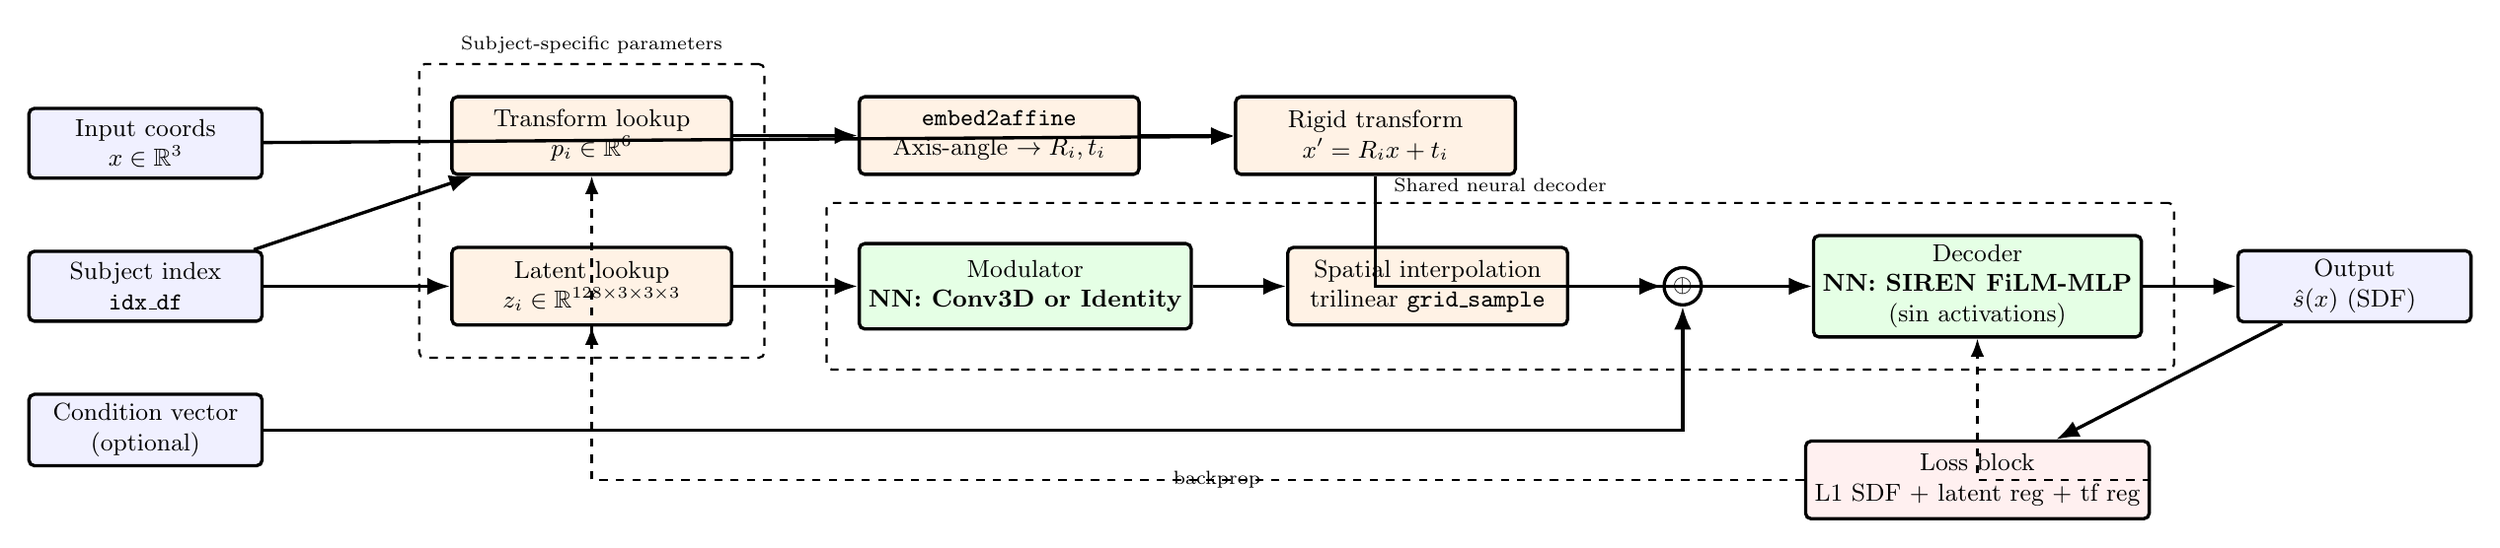
\begin{tikzpicture}[
    node distance=9mm and 12mm,
    >=Latex,
    block/.style={draw, rounded corners=2pt, align=center, minimum width=34mm, minimum height=10mm, font=\small, very thick},
    io/.style={draw, rounded corners=2pt, align=center, minimum width=30mm, minimum height=9mm, font=\small, very thick, fill=blue!6},
    op/.style={draw, rounded corners=2pt, align=center, minimum width=36mm, minimum height=10mm, font=\small, very thick, fill=orange!10},
    nn/.style={draw, rounded corners=2pt, align=center, minimum width=40mm, minimum height=11mm, font=\small, very thick, fill=green!10},
    sum/.style={draw, circle, inner sep=1.5pt, font=\small, very thick},
    group/.style={draw, rounded corners=2pt, thick, dashed, inner sep=4mm}
]

% Inputs
\node[io] (coords) {Input coords\\$x\in\mathbb{R}^3$};
\node[io, below=of coords] (sid) {Subject index\\\texttt{idx\_df}};
\node[io, below=of sid] (cond) {Condition vector\\(optional)};

% Subject-specific params
\node[op, right=24mm of sid] (latents) {Latent lookup\\$z_i\in\mathbb{R}^{128\times3\times3\times3}$};
\node[op, above=of latents] (tflkup) {Transform lookup\\$p_i\in\mathbb{R}^{6}$};

% Transform path
\node[op, right=16mm of tflkup] (embed) {\texttt{embed2affine}\\Axis-angle $\rightarrow R_i,t_i$};
\node[op, right=of embed] (rigid) {Rigid transform\\$x' = R_i x + t_i$};

% Latent path
\node[nn, right=16mm of latents] (mod) {Modulator\\\textbf{NN: Conv3D or Identity}};
\node[op, right=of mod] (gs) {Spatial interpolation\\trilinear \texttt{grid\_sample}};
\node[sum, right=of gs] (concat) {$\oplus$};

% Decoder and output
\node[nn, right=14mm of concat] (siren) {Decoder\\\textbf{NN: SIREN FiLM-MLP}\\(sin activations)};
\node[io, right=of siren] (sdf) {Output\\$\hat{s}(x)$ (SDF)};

% Losses
\node[block, below=13mm of siren, fill=red!6] (loss) {Loss block\\L1 SDF + latent reg + tf reg};

% Group boxes
\node[group, fit=(latents)(tflkup), label={[font=\scriptsize]north:Subject-specific parameters}] {};
\node[group, fit=(mod)(siren), label={[font=\scriptsize]north:Shared neural decoder}] {};

% Arrows
\draw[->, very thick] (coords) -- (rigid);
\draw[->, very thick] (sid) -- (latents);
\draw[->, very thick] (sid) -- (tflkup);
\draw[->, very thick] (tflkup) -- (embed);
\draw[->, very thick] (embed) -- (rigid);
\draw[->, very thick] (latents) -- (mod);
\draw[->, very thick] (mod) -- (gs);
\draw[->, very thick] (gs) -- (concat);
\draw[->, very thick] (cond) -| (concat);
\draw[->, very thick] (rigid) |- (siren);
\draw[->, very thick] (concat) -- (siren);
\draw[->, very thick] (siren) -- (sdf);
\draw[->, very thick] (sdf) -- (loss);
\draw[->, dashed, thick] (loss.west) -| node[pos=0.22,left,font=\scriptsize]{backprop} (latents.south);
\draw[->, dashed, thick] (loss.west) -| (tflkup.south);
\draw[->, dashed, thick] (loss.east) -| (siren.south);

\end{tikzpicture}
\caption{CINeMA-Bone forward architecture. Neural blocks are explicitly labeled: Conv3D modulator and SIREN (sinusoidal MLP with FiLM-style modulation).}
\label{fig:architecture}
\end{figure}

\section{Loss Function and Regularization}
Implementation: \texttt{utils.py} (\texttt{BoneLoss}).

Current training objective:
\begin{equation}
\mathcal{L}=\mathcal{L}_{\text{SDF}} + \lambda_z\|z\|_2^2 + \lambda_t\|p\|_2^2.
\end{equation}

In current default setup:
\begin{itemize}[leftmargin=*]
    \item $\mathcal{L}_{\text{SDF}}$: L1 reconstruction loss,
    \item latent regularization active,
    \item transform regularization active if weight is set,
\end{itemize}

\section{Optimization Setup}
Implementation: \texttt{build\_bone\_atlas.py}.

Parameter groups have separate learning rates:
\begin{itemize}[leftmargin=*]
    \item decoder weights,
    \item latent codes,
    \item rigid transforms.
\end{itemize}

Optimizer is AdamW; scheduler is cosine annealing when enabled. Mixed precision (AMP) is supported.

\section{Training Procedure (Step-by-Step)}
\subsection{Inputs per Batch}
The dataloader returns:
\begin{itemize}[leftmargin=*]
    \item \texttt{coords}: sampled coordinates,
    \item \texttt{values}: ground-truth SDF at those coordinates,
    \item \texttt{conditions}: condition vectors,
    \item \texttt{idx\_df}: subject indices (for latent/transform lookup).
\end{itemize}

\subsection{One Inner Training Update}
For each chunk of sampled points:
\begin{enumerate}[leftmargin=*]
    \item Fetch subject latent and transform using \texttt{idx\_df}.
    \item Transform coordinates by subject rigid transform.
    \item Interpolate subject latent features at transformed coordinates.
    \item Run SIREN decoder to predict SDF.
    \item Compute loss terms.
    \item Backpropagate and update parameters.
\end{enumerate}

\subsection{Epoch-Level Behavior}
Each epoch reports:
\begin{itemize}[leftmargin=*]
    \item total loss,
    \item SDF loss,
    \item latent regularization,
    \item transform regularization,
    \item rolling average total loss.
\end{itemize}

Validation checkpoints trigger reconstruction exports and model checkpoints.

\section{Inference Procedure (How Atlas Is Produced)}
There are two inference modes.

\subsection{Mode A: Subject Reconstruction}
Goal: reconstruct a specific subject.
\begin{enumerate}[leftmargin=*]
    \item Generate a dense 3D grid of atlas/world coordinates.
    \item Use that subject's latent code and transform.
    \item Decode SDF on all grid points (chunked inference to avoid OOM).
    \item Reshape to 3D volume.
    \item Save NIfTI and extract mesh via marching cubes.
\end{enumerate}

\subsection{Mode B: Population Atlas Generation}
Goal: produce the canonical mean atlas.
\begin{enumerate}[leftmargin=*]
    \item Compute mean latent code across training subjects:
    \begin{equation}
    \bar{z}=\frac{1}{N}\sum_{i=1}^{N} z_i.
    \end{equation}
    \item Use zero condition vector and no subject-specific transform.
    \item Decode SDF on dense world grid.
    \item Save atlas SDF volume and extract zero-level mesh.
\end{enumerate}

This atlas mesh is the final population-level shape model.

\section{Fracture Density Map Generation}
Implementation: \texttt{fracture\_atlas/density\_map.py}, \texttt{fracture\_atlas/fracture\_analyzer.py}.

Procedure:
\begin{enumerate}[leftmargin=*]
    \item Load trained model and regenerate atlas SDF.
    \item For each subject, infer subject SDF on same atlas grid.
    \item Detect atlas-subject discrepancies near/in bone volume as fracture indicators.
    \item Accumulate indicators across subjects.
    \item Normalize by number of subjects to get voxelwise fracture density.
\end{enumerate}

Additional outputs:
\begin{itemize}[leftmargin=*]
    \item fracture density volume (NIfTI/NumPy),
    \item colored atlas overlay mesh,
    \item high-density zone masks and meshes,
    \item CAD-exportable iso-surfaces.
\end{itemize}

\section{Why Latent Codes and Transforms Are Both Needed}
\textbf{Transforms} solve alignment (pose/location differences).  \\
\textbf{Latent codes} solve morphology (true shape differences).

If only transforms were used, model could align bones but not capture subject-specific anatomical variation.  \\
If only latent codes were used, model would waste latent capacity to encode pose instead of anatomy.

Jointly learning both makes the atlas cleaner and the latent space more meaningful.

\section{Current Default Configuration Summary}
\begin{itemize}[leftmargin=*]
    \item Input representation: per-subject 3D SDF volumes.
    \item Decoder: SIREN-based implicit network with latent modulation.
    \item Subject parameters: latent tensor + 6-DoF transform.
    \item Loss: L1 SDF + latent regularization (+ transform regularization if weighted).
    \item Atlas output: mean-latent decoded SDF and mesh.
\end{itemize}

\section{Operational Pipeline (Step-by-Step)}
This section gives a practical implementation-level walkthrough of how outputs are produced in this repository.

\subsection{Stage 1: Precompute Subject SDF Volumes}
\begin{enumerate}[leftmargin=*]
    \item Run preprocessing (\texttt{run.py --prepare-data} or \texttt{data\_loading/prepare\_data.py}).
    \item For each subject folder, discover all STL fragment files.
    \item Merge fragments into one mesh for that subject.
    \item Center and scale mesh to normalized coordinates.
    \item Voxelize mesh to occupancy and convert occupancy to SDF.
    \item Save subject SDF as \texttt{data/processed/<subject>\_sdf.npy}.
\end{enumerate}

\subsection{Stage 2: Build Training Samples Each Epoch}
\begin{enumerate}[leftmargin=*]
    \item Load each subject's SDF volume in \texttt{BoneDataset}.
    \item Sample coordinates in two streams:
    \begin{itemize}[leftmargin=*]
        \item near-surface samples for boundary accuracy,
        \item uniform samples for global shape coverage.
    \end{itemize}
    \item Return tensors: coordinates, SDF targets, optional conditions, and subject indices.
\end{enumerate}

\subsection{Stage 3: Forward Pass for One Sample Chunk}
\begin{enumerate}[leftmargin=*]
    \item Use subject index to fetch that subject's latent code and transform parameters.
    \item Convert transform embedding to affine form and transform coordinates to subject-aligned space.
    \item Pass latent code through modulator block (Conv3D or identity).
    \item Interpolate modulated latent features at transformed coordinates using trilinear sampling.
    \item Concatenate optional conditions.
    \item Decode with shared SIREN to predict SDF values.
\end{enumerate}

\subsection{Stage 4: Loss and Parameter Update}
\begin{enumerate}[leftmargin=*]
    \item Compute SDF reconstruction loss (L1).
    \item Add latent-code regularization and transform regularization if configured.
    \item Backpropagate total loss.
    \item Update shared decoder weights and all subject-specific parameters (latents/transforms) via AdamW.
\end{enumerate}

\subsection{Stage 5: Validation and Checkpointing}
\begin{enumerate}[leftmargin=*]
    \item At validation intervals, generate:
    \begin{itemize}[leftmargin=*]
        \item atlas reconstruction,
        \item sample train/val subject reconstructions.
    \end{itemize}
    \item Save NIfTI SDF volumes and STL meshes.
    \item Save model checkpoint containing decoder weights, latents, transforms, and config.
\end{enumerate}

\subsection{Stage 6: Atlas Synthesis (Inference)}
\begin{enumerate}[leftmargin=*]
    \item Compute mean latent code over training subjects.
    \item Decode mean latent on dense 3D world grid.
    \item Extract zero level set to obtain atlas mesh.
    \item Save atlas SDF and mesh as canonical population shape.
\end{enumerate}

\subsection{Stage 7: Fracture Density Map Generation}
\begin{enumerate}[leftmargin=*]
    \item Load trained checkpoint.
    \item Recompute atlas SDF on common grid.
    \item Reconstruct each subject SDF on the same grid.
    \item Compute atlas-subject discrepancy indicators in/near bone surface.
    \item Accumulate across subjects and normalize by subject count.
    \item Save fracture density volume, overlay mesh, high-density zones, and CAD exports.
\end{enumerate}

\section{Practical Reading Guide for New Readers}
If someone is new to this model, read in this order:
\begin{enumerate}[leftmargin=*]
    \item \texttt{data\_loading/mesh\_to\_volume.py} and \texttt{prepare\_data.py} (how input is constructed),
    \item \texttt{data\_loading/dataset.py} (what the trainer actually sees),
    \item \texttt{models/inr\_decoder.py} and \texttt{models/siren.py} (forward model),
    \item \texttt{build\_bone\_atlas.py} (optimization and atlas generation),
    \item \texttt{fracture\_atlas/*.py} (downstream fracture analytics).
\end{enumerate}

\end{document}
